\section{Equation of motion for grains with radiation, gas drag, and
  magnetic field}
\label{sec:equat-moti-grains}

Following \citet{Draine:1979a}, the drag force on a grain that is
moving at relative velocity \(\bm{w} = \bm{v}\grain - \bm{v}\gas\)
through a partially ionized gas can be written as a sum over each
collider species, \(k\), with mass \(m_k\), abundance relative to
hydrogen \(\alpha_k\) and charge \(z_k\). If the relative speed,
\(w = \abs{\bm{w}}\), is normalized to the thermal speed of each
species:
\begin{equation}
  \label{eq:s-velocity}
  s_k = \left( m_k w^2 / 2 k T  \right)^{1/2} \ ,
\end{equation}
then the magnitude of the force is 
\begin{equation}
  \label{eq:ds79}
  f\drag = f_* \sum_k \alpha_k \left[ G_0(s_k) + z_k^2 \phi^2 \ln(\Lambda/z_k) G_2(s_k) \right],
\end{equation}
where \(f_*\) is a characteristic thermal force on the grain (see
eq.~[\ref{eq:fstar}]). The dimensionless functions of normalized speed
\(G_0(s)\) and \(G_2(s)\) are given by
\begin{align}
  \label{eq:G0}
  G_0(s) & = \left( s^2 + 1 - \frac{1}{4 s^2} \right) \erf(s)
  +  \left( s + \frac{1}{2 s} \right) \frac{e^{-s^2}}{\sqrt{\pi}}\\
  \label{eq:G2}
  G_2(s) & = \frac{\erf(s)}{s^2} - \frac{2 e^{-s^2}}{s \sqrt{\pi}} \ .
\end{align}
The \(G_0\) term is due to inelastic solid-body collisions in the
Epstein limit, and is derived in \S~4 of \citet{Baines:1965a}.  The
\(G_2\) term is due to electrostatic Coulomb interactions, with
\(\phi\) being the grain potential in thermal units
(eq.~[\ref{eq:phi-potential}]) and \(\Lambda\) the plasma parameter.  It was
first derived in the different context of dynamical friction in
stellar systems by \citet{Chandrasekhar:1941a}.
Figures~\ref{fig:drag-components}--\ref{fig:gas-grain-drag-photoionized}
show example applications to gas--grain drag in a photoionized region.

The grain trajectories presented in \S~\ref{sec:grain-traj-along} and
\ref{sec:grain-traj-with} are calculated by numerically solving the
grain equation of motion:
\begin{equation}
  \label{eq:grain-equation-motion}
  m\grain \frac{d^2 \bm{r}}{d t^2} = \bm{f} \ .
\end{equation}
The total force \(\bm{f}\) is the sum of radiation, drag, and Lorentz
terms:
\begin{equation}
  \label{eq:total-force}
  \bm{f} = \frac{\sigma\grain \Qp L}{4\pi R^2 c} \hat{\bm{r}}
  - f\drag \hat{\bm{w}}
  + \frac{z\grain e}{c} \bm{w} \times \bm{B} \ ,
\end{equation}
with \(f\drag\) given by equation~\eqref{eq:ds79} and where
\(\hat{\bm{r}}\) is the unit vector in the radial direction and
\(\hat{\bm{w}} = \bm{w} / w\) is the unit vector along the direction
of gas--grain relative motion.  In the strong magnetic coupling limit
(see \S~\ref{sec:grain-traj-with} and \ref{sec:tight-magn-coupl}), the
Lorentz term is not included explicitly, but instead the equation of
motion is solved for the guiding center by replacing \(\bm{f}\) by its
projection along the magnetic field: 
\begin{equation}
  \label{eq:projected-force}
  \widetilde{\bm{f}} = (\bm{f} \cdot \hat{\bm{b}})  \, \hat{\bm{b}} \ ,
\end{equation}
where \(\hat{\bm{b}} = \bm{B} / B\).

If distances are measured in units of the radiative turnaround radius,
\(R\starstar\) (eq.~[\ref{eq:dust-r0}]), and times in units of
\(R\starstar / v_\infty\), then the grain acceleration
\(\bm{a}\grain = \bm{f} / m\grain\) in the non-magnetic case can be
written in non-dimensional form as
\begin{equation}
  \label{eq:grain-accelration}
  \frac{\bm{a}\grain}{a\starstar}
  = \frac{R\starstar^2}{2 R^{2}} \hat{\bm{r}}
  - C\drag \frac{f\drag}{f_*} \hat{\bm{w}} \, 
\end{equation}
where \(a\starstar = v_\infty^2 / R\starstar\) is a characteristic
acceleration scale and the dimensionless drag constant is
\begin{equation}
  \label{eq:drag-constant}
  C\drag = \frac{4}{\Qp} \left(\frac{\sound \tau_* \kappa\grain}{v_\infty \kappa}\right)^2 \ .
\end{equation}

A collection of python programs that implement the equations of this
appendix is available at
\url{https://github.com/div-B-equals-0/dust-trajectories}, including
programs to generate all the grain trajectory figures of this paper
plus additional figures and movies.  The integration of
equation~\eqref{eq:grain-equation-motion} is carried out using the
python library function \texttt{scipy.integrate.odeint}, which wraps
the Fortran ODEPACK library \citep{Hindmarsh:1983a, Jones:2001a}.

% \begin{figure}
%   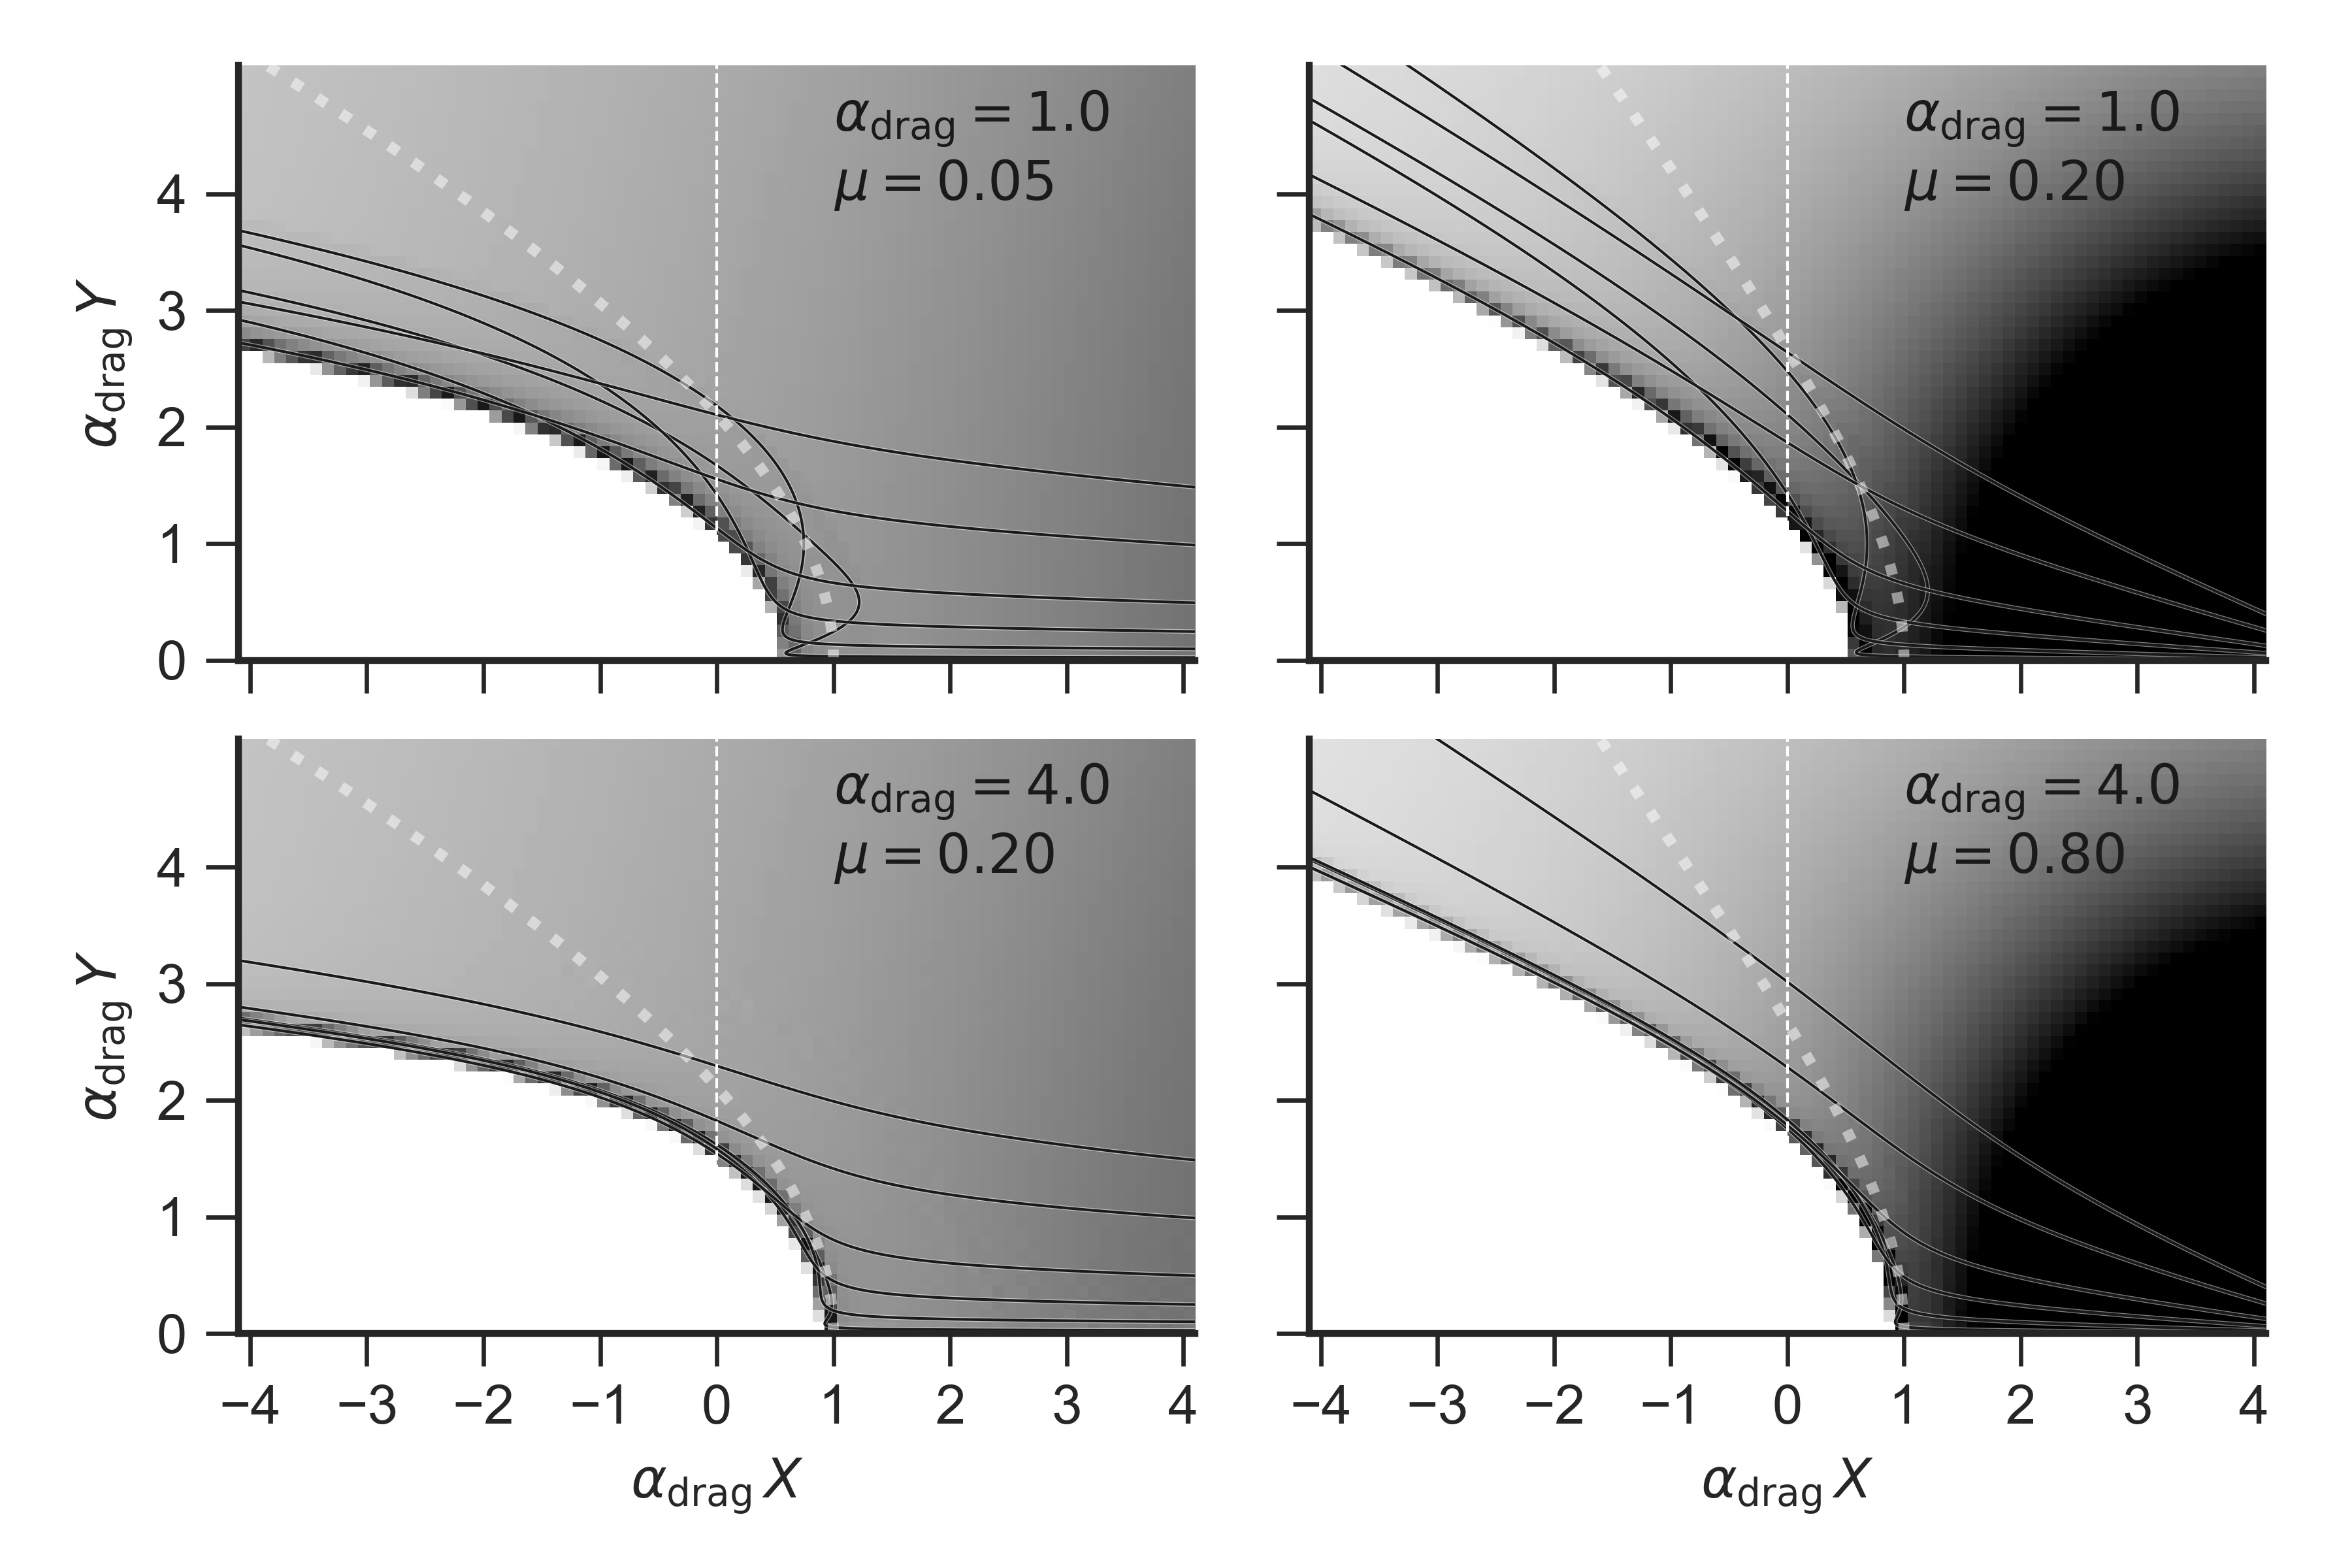
\includegraphics[width=\linewidth]{figs/dust-couple-div-stream}
%   \caption{Divergent dragoids}
%   \label{fig:divergent-dragoids}
% \end{figure}

% To find the dust grain trajectories \(R\grain(\theta)\) in the presence of
% radiation and drag forces (\S~\ref{sec:bow-wave-drag}), we numerically
% integrate the equations of motion. We define dimensionless cylindrical
% polar coordinates,
% \begin{equation}
%   \label{eq:dust-XY}
%   (X, Y) = \left(\frac{R\grain(\theta) \cos\theta } {R_0}, \ 
%     \frac{R\grain(\theta) \sin\theta } {R_0}\right)
%   \ ,
% \end{equation}
% and dust grain velocities,
% \begin{equation}
%   \label{eq:dust-UV}
%   (U, V) = \left( \frac{\bm{v}\grain \cdot \uvec{x}} {v_\infty}, \ 
%   \frac{\bm{v}\grain \cdot \uvec{y}} {v_\infty}\right) \ ,
% \end{equation}
% where \(\uvec{x}\) and \(\uvec{y}\) are unit vectors along the \(X\)
% and \(Y\) axes (parallel and perpendicular, respectively, to the
% symmetry axis).  The grain equation of motion then follows from
% equations~(\ref{eq:dust-rad-force}, \ref{eq:dust-r0},
% \ref{eq:dust-fdrag}--\ref{eq:dust-alpha}) as the following set of
% coupled differential equations:
% \begin{gather}
%   \label{eq:dust-motion}
%   \begin{aligned}
%     \frac{d X}{d t} &= U \quad\quad
%     \frac{d Y}{d t} = V \\
%     \frac{d U}{d t} &= \frac12 \left[  
%       X \left(X^2 + Y^2\right)^{-3/2} - \alpha\drag^2 D_1 \left(U - U_1\right)
%     \right] \\
%     \frac{d V}{d t} &= \frac12 \left[  
%       Y \left(X^2 + Y^2\right)^{-3/2} - \alpha\drag^2 D_1 \left(V - V_1\right)
%     \right] \ ,
%   \end{aligned}
% \end{gather}
% where \((U_1, V_1)\) are the components of the gas velocity (assumed
% fixed), given by
% \begin{equation}
%   \label{eq:dust-gas-velocities}
%   (U_1, V_1) = 
%   \begin{cases}
%     \text{parallel stream} & (-1, 0)\\
%     \text{divergent stream} &
%     \left( \dfrac{X - \mu^{-1}}{R_1},\ \dfrac{Y}{R_1}\right) \ ,
%   \end{cases}
% \end{equation}
% where
% \begin{equation}
%   \label{eq:dust-R1}
%   R_1 = \left( \bigl(X - \mu^{-1}\bigr)^2 + Y^2 \right)^{1/2}
% \end{equation}
% is the distance from the second source, located at
% \((X, Y) = (\mu^{-1}, 0)\).  The dimensionless gas density, \(D_1\),
% normalized by the value at \((X, Y) = (1, 0)\), is
% \begin{equation}
%   \label{eq:dust-gas-density}
%   D_1 = 
%   \begin{cases}
%     \text{parallel stream} & 1\\
%     \text{divergent stream} & \dfrac{\bigl(\mu^{-1} - 1\bigr)^2} {R_1^{2}} \ .
%   \end{cases}
% \end{equation}

% Equations~\eqref{eq:dust-motion} are integrated using the python
% wrapper \texttt{scipy.integrate.odeint} to the Fortran ODEPACK library
% \citep{Hindmarsh:1983a, Jones:2001a}, with results shown in
% Figure~\ref{fig:dust-wave-coupling} for parallel-stream cases and
% Figure~\ref{fig:divergent-dragoids} for divergent-stream cases. 

%%% Local Variables:
%%% mode: latex
%%% TeX-master: "dusty-bow-wave"
%%% End:
